\documentclass{article}
% Útgáfa 1.5

% pakkar fyrir töflur; array er notað í "math-mode"; arydshln fyrir brotalínur í töflum
\usepackage{array,tabularx}%,arydshln}  
% íslenskt letur, orðaskiptingar ...
\usepackage[english]{babel}
\usepackage[T1]{fontenc}
% númera jöfnur, töflur, myndir, ...
\usepackage{enumerate}
% fyrir krækjur
\usepackage[colorlinks,linkcolor=blue,citecolor=blue,urlcolor=blue]{hyperref}
% ýmis tákn, leturgerðir, ... ATH amsmath fyrir \text{} skipunina
\usepackage{amsmath,amssymb,euscript}   
% til að setja inn *.eps myndir ef við notum dvi og ps skjöl...
\usepackage{epsfig}    % \epsfig{...}
% ... en ef við notum pdf beint, þá er þetta pakkinn sem við þurfum
\usepackage{graphicx}  % \includegraphics[...]{...}
% litamöguleikar fyrir texta
\usepackage{color}
% til þess að myndir og töflur standi þar sem þær eiga að standa!
\usepackage{here}
%
\setlength{\textwidth}{7in}
\setlength{\textheight}{9in}
\setlength{\headheight}{0in}
\setlength{\headsep}{6pt}
\setlength{\topskip}{0in}
\setlength{\topmargin}{0cm}
\setlength{\oddsidemargin}{-0.3in}
\setlength{\marginparwidth}{10pt}
% dregur fyrstu línu í hverri málsgrein inn - nota 0cm fyrir engan inndrátt fyrir allar málsgreinar en \noindent í upphafi málsgreinar til að hafa engan inndrátt í þeirri málsgrein einni:
\setlength{\parindent}{0cm}
% viljum hafa eitt línubil milli efnisgreina
\setlength{\parskip}{1.5ex plus 0.75ex minus 0.5ex}
% 1.5 í línubil
\renewcommand{\baselinestretch}{1.025}

% Environments
\newenvironment{alist}[1][$\quad\,$1.]{
\vspace*{-8pt} \begin{enumerate}[label=\alph*),itemsep=4pt,parsep=3pt]}
{\end{enumerate}\vspace*{-3pt}}

\newenvironment{ttafla}[1][$\quad\,$1.]{
\begin{tabular}{rcl} \renewcommand\arraystretch{2} }
{\end{tabular}}



%Bætt við af mér (Hannesi)
% Þjappa saman
\widowpenalty=600
\clubpenalty=600
\usepackage[compact]{titlesec}
\titlespacing{\section}{0pt}{2ex plus 0.75ex minus 0.75ex}{1ex plus 0.3ex minus 0.3ex}
\titlespacing{\subsection}{0pt}{1ex plus 0.25ex minus 0.25ex}{0ex plus 0.1ex minus 0.1ex}
\titlespacing{\subsubsection}{0pt}{0.5ex plus 0.1ex minus 0.1ex}{0ex plus 0.1ex minus 0.1ex}

% Bolda caption
\usepackage[hang,small,bf]{caption}

% Efnaformúlur og myndir
%\usepackage[version=3]{mhchem}
\usepackage{chemfig}

% Komma í stað punkts
\usepackage{icomma}

% Annað
\usepackage{subfig}
\usepackage{array}
\usepackage{bigstrut}
\usepackage{multirow}
\usepackage{multicol}
\usepackage{enumerate}
%\usepackage{enumitem}
\usepackage{wrapfig}
\newcommand{\HRule}{\rule{\linewidth}{0.5mm}}
\usepackage{ulem}
%\usepackage[thinspace,mediumqspace,amssymb]{SIunits}

%Tikz
\usepackage{tikz}
\usetikzlibrary{fit,arrows,decorations.pathmorphing,decorations.text,backgrounds,positioning,fit,petri,3d,calc}
%% 3d hnitakerfi
\usepackage{tikz-3dplot}
\tdplotsetmaincoords{75}{130}
%\begin{tikzpicture}[scale=5,tdplot_main_coords]
%
%%set up some coordinates 
%%-----------------------
%\coordinate (O) at (0,0,0);
%
%%determine a coordinate (P) using (r,\theta,\phi) coordinates.  This command
%%also determines (Pxy), (Pxz), and (Pyz): the xy-, xz-, and yz-projections
%%of the point (P).
%%syntax: \tdplotsetcoord{Coordinate name without parentheses}{r}{\theta}{\phi}
%\tdplotsetcoord{P}{\rvec}{\thetavec}{\phivec}


%%%%%%%%%%%%%%% SKIPANIR %%%%%%%%%%%%%%%%%%%%%%%%
%% LITASTYTTINGAR
%
\definecolor{dgreen}{rgb}{0,0.8,0}
\newcommand{\red}[1]{{\color{red} #1}}
\newcommand{\green}[1]{{\color{dgreen} #1}}
\newcommand{\blue}[1]{{\color{blue} #1}}
\newcommand{\black}[1]{{\color{black} #1}}
%
% ALLS KYNS STÆRÐFRÆÐIDÓT
%
\newcommand{\lvec}{\overrightarrow}
%
% ýmsar diffurstyttingar
\newcommand{\dif}{\,\mathrm{d}}
\newcommand{\dx}{\,\mathrm{d}x}
\newcommand{\dy}{\,\mathrm{d}y}
\newcommand{\dz}{\,\mathrm{d}z}
\newcommand{\dt}{\,\mathrm{d}t}
% afleiður og hlutafleiður
\renewcommand{\d}[2]{\frac{\dif{#1}}{\dif{#2}}}
\newcommand{\dd}[3]{\frac{\dif^{#1}{#2}}{\dif^{#1}{#3}}}
\newcommand{\p}[2]{\frac{\partial{#1}}{\partial {#2}}}
\newcommand{\pp}[3]{\frac{\partial^{#1}{#2}}{\partial{#3}^{#1}}}
%
% bil, millistig \; og \quad
\newcommand{\bil}{\hspace*{6pt}}
\newcommand{\Bil}{\hspace*{10pt}}
\newcommand{\vbil}{\vspace*{-6pt}}
\newcommand{\vBil}{\vspace*{-10pt}}

% samasemmerki með aukaplássi á báða bóga
\newcommand{\bils}{\bil=\bil}
%
\newcommand{\bc}{\begin{center}}
\newcommand{\ec}{\end{center}}
%
\newcommand{\beq}{\begin{equation}}
\newcommand{\eeq}{\end{equation}}
%
\newcommand{\beqa}{\begin{eqnarray*}}
\newcommand{\eeqa}{\end{eqnarray*}}
%
\newcommand{\ba}{\begin{array}}
\newcommand{\ea}{\end{array}}
%
\newcommand{\bma}{\begin{matrix}}
\newcommand{\ema}{\end{matrix}}
%
\newcommand{\bmh}{\left[\begin{matrix}}
\newcommand{\emh}{\end{matrix}\right]}
%
\newcommand{\ts}{\textstyle}
\newcommand{\ds}{\displaystyle}

% Frá mér (Hannesi)
\newcommand{\lausn}{\textbf{\textit{Lausn:}}}
\newcommand{\solution}{\textbf{\textit{Solution:}}}
\newcommand{\daemi}{\textbf{\textit{Dæmi:}}}
\newcommand{\bt}{\begin{table}[H]}
\newcommand{\et}{\end{table}}
\newcommand{\atm}{\text{atm}}
\newcommand{\calories}{\text{cal}}
\everymath{\displaystyle} % Svo allar jöfnur taka aldrei minna pláss
\renewcommand\tabcolsep{2pt} % Bil dalka í töflum
\setlength{\arraycolsep}{1.5pt}
%\usepackage{fancyhdr}
%\setlength{\headheight}{25pt}
%\pagestyle{fancy}
%\renewcommand{\headrulewidth}{0.4pt}
%\renewcommand{\footrulewidth}{0.4pt}
%\usepackage[top=2.5in, bottom=1.5in, left=1in, right=1in]{geometry}
\usepackage{amssymb}
\usepackage{pifont}
\newcommand{\cmark}{\text{\ding{51}}}%
\newcommand{\xmark}{\text{\ding{55}}}%

\usepackage{pbox}
%\usepackage{fancyvrb}
\usepackage{array}
\newcolumntype{L}[1]{>{\raggedright\let\newline\\\arraybackslash\hspace{0pt}}m{#1}}
\newcolumntype{C}[1]{>{\centering\let\newline\\\arraybackslash\hspace{0pt}}m{#1}}
\newcolumntype{R}[1]{>{\raggedleft\let\newline\\\arraybackslash\hspace{0pt}}m{#1}}
\usepackage[utf8]{inputenc}
\usepackage{framed}
\usepackage{paralist}
\renewenvironment{enumerate}[1]{\begin{compactenum}#1}{\end{compactenum}}
\usetikzlibrary{shapes.multipart,positioning,arrows}

\begin{document}
\begin{titlepage}
\begin{center}
\textsc{}\\[2cm] 


\includegraphics[width=6cm]{Haskoli_Islands_rett.jpg}\\[0.5cm]

\HRule \\[0.6cm]
{ \huge \bfseries Group assignment 2: Class diagram}\\[0.2cm]
\HRule \\[0.4cm]

\textsc{\normalsize Þróun hugbúnaðar} \\
\textsc{Spring 2015} \\[1.5cm]

\begin{minipage}{0.45\textwidth}
\begin{flushleft} \large
\textit{Students:} (Group F2a)\\
\textsc{Einar Helgi Þrastarson} \\
\textsc{Hannes Pétur Eggertsson} \\
\textsc{Sigurður Birkir Sigurðsson} \\
\end{flushleft}
\end{minipage}
\begin{minipage}{0.45\textwidth}
\begin{flushright} \large
\textit{Teachers:} \\
\textsc{Matthias Book}\\
\textsc{Kristín Fjóla Tómasdóttir}\\
\textsc{ }\\
\end{flushright}
\end{minipage}

\end{center}
\end{titlepage}


% Description of the project
\section{Introduction}
In this document there's the class diagram for group F2a. Group members are: Einar Helgi Þrastarson (personal ID number: 110287-2919), Hannes Pétur Eggertsson (240889-2939) and Sigurður Birkir Sigurðsson (120589-2539). Our project is to build an user interface for a fantasy football game. In our class diagram we felt it made sense to split the classes into two categories, back-end classes and front-end classes. In the appendix we put our current idea how the UI will look like when the game is ready. The presenter on Wednesday, March 4th 2015, will be Hannes Pétur Eggertsson.

\subsection{Notation}
In our class diagrams we use the following notation:\vspace*{-0.3cm}
\begin{itemize}\itemsep-4pt
\item[--] means a private variable or method (not directly accessable by other classed).
\item[+] means a public variable or method (directly accessable by other methods).
\end{itemize}

\tikzset{umlclass/.style={
        draw=black,fill=yellow!16,rectangle split,align=center, rectangle split part align={center,left}, minimum width=4cm,rounded corners},draw,rectangle split parts=4}

Also, each class in the diagram has four sections:
\begin{center} \vspace*{-0.15cm}
\begin{tikzpicture}
\begin{scope}[xshift=8cm,yshift=0cm]
\node[umlclass] (t1)
 {\textbf{\large \textit{The class' name.}}
 \nodepart{two}
  {\footnotesize
  \begin{tabular}{l} 
   Short description of the class.
  \end{tabular}}
 \nodepart{three}
  \begin{tabular}{l}
  The class' variables and their type listed\\
  on the format:\\
   --/+ \texttt{type1 variable1}\\
   --/+ \texttt{anotherClass variable2}\\
  \end{tabular}
 \nodepart{four}
  \begin{tabular}{l}
   The class' methods listed on the format:\\
   --/+ \texttt{type1 method1(type variable,...)}\\
   --/+ \texttt{type2 method2(...)}\\
  \end{tabular}
 };
\end{scope}
\end{tikzpicture}
\end{center}\vspace*{-0.15cm}
If the class wasn't created by us it is filled with red. Classes are then connected using arrows:

\begin{tikzpicture}
\draw[arrows={-angle 60},thick] node[left]{Class A} (0,0) to (3,0)node[draw=none,midway,above=0cm] {\hspace*{3cm}\textit{uses}} node[right]{Class B};
\begin{scope}[yshift=-0.8cm]
\draw[arrows={-open triangle 60},thick] node[left]{Class A} (0,0) to (3,0)node[draw=none,midway,above=0cm] {\hspace*{3cm}\textit{extends}} node[right]{Class B};
\end{scope}
\begin{scope}[yshift=-1.6cm]
\draw[arrows={-triangle 60},thick] node[left]{Class A} (0,0) to (3,0)node[draw=none,midway,above=0cm] {\hspace*{3cm}\textit{implements}} node[right]{Class B};
\end{scope}
\end{tikzpicture}

In most cases we can tell how many classes 'Class A' and 'Class B' will be associated with, this is shown by placing an arrow at the beginning and end of an arrow, e.g.

\begin{tikzpicture}
\draw[arrows={-angle 60},thick] node[left]{Class A} node[above right]{1} (0,0) to (3,0)node[draw=none,midway,above=0cm] {\hspace*{3cm}\textit{uses}} node[above left]{0--10} node[right]{Class B};
\end{tikzpicture}

if each instance of 'Class A' will use 'Class B' in a range of 0 to 10 instances.

\subsection{Terminologies and Concepts}
\paragraph{User} A (human) user actually playing the game.
\paragraph{Player} A football player in the game, e.g. Gylfi Sigurðsson.
\paragraph{Team} A football team in the game, e.g. Manchester United.
\paragraph{Roster} The user's bought players, the players could be from multiple teams. Note that the roster includes both players which user has set on and off the field. A roster can have up to 15 players.

\section{Class diagram}
We decided to split our class diagram into two figures: \textbf{Back-end classes} and \textbf{Front-end classes}. The back-end classes take care of storing and keeping track of all information as the game is running. The front-end classes take care of displaying the information to the users playing the game as well as handling their input.
\subsection{Back-end classes}
\begin{tikzpicture}
%% ==========================================
%% User
%% ==========================================
\begin{scope}[yshift=-6cm]
\node[umlclass] (user)
 {\textbf{\large \textit{User}}
 \nodepart{two}
  {\footnotesize
  \begin{tabular}{l} 
   This class keeps track of all information about\\
   each user playing the game.\\
   
  \end{tabular}}
 \nodepart{three}
  \begin{tabular}{l}
   -- \texttt{int money}\\
   -- \texttt{int score}\\
   -- \texttt{String name}\\
   -- \texttt{Roster roster}\\
  \end{tabular}
 \nodepart{four}
  \begin{tabular}{l}
   + \texttt{void User(String name, Roster r)}\\
   + \texttt{boolean changeMoney(int dMoney)}\\
   + \texttt{void changeScore(int dScore)}\\
   + \texttt{String getName()}\\
   + \texttt{Roster getRoster()}\\
   + \texttt{void addScoresToStats()}
  \end{tabular}
 };
\end{scope}

%% ==========================================
%% Roster
%% ==========================================
\begin{scope}[xshift=9.5cm,yshift=0.7cm]
\node[umlclass] (roster)
 {\textbf{\large \textit{Roster}}
 \nodepart{two}
  {\footnotesize
  \begin{tabular}{l} 
   Keeps track of which football players are in which user team/roster.
  \end{tabular}}
 \nodepart{three}
  \begin{tabular}{l}
   -- \texttt{Player[2] goalkeepers}\\
   -- \texttt{Player[2] goalkeepersOnField}\\
   -- \texttt{Player[5] defenders}\\
   -- \texttt{Player[5] defendersOnField}\\
   -- \texttt{Player[5] midfielders}\\
   -- \texttt{Player[5] midfieldersOnField}\\
   -- \texttt{Player[3] strikers}\\
   -- \texttt{Player[3] strikersOnField}\\
   -- \texttt{Player captain}\\
   -- \texttt{int numberOfPlayersOnField}\\
  \end{tabular}
 \nodepart{four}
  \begin{tabular}{l}
   + \texttt{Roster()}\\
   + \texttt{void removePlayerFromTeam(Player player)}\\
   + \texttt{boolean addPlayerToTeam(Player player)}\\
   + \texttt{void changeCaptain(Player newCaptain)}\\
   + \texttt{boolean putPlayerOnField(Player player)}\\
   + \texttt{boolean removePlayerFromField(Player player)}\\
  \end{tabular}
 };
\end{scope}

%% ==========================================
%% MainGame
%% ==========================================
\begin{scope}[xshift=0cm,yshift=1.5cm]
\node[umlclass] (maingame)
 {\textbf{\large \textit{MainGame}}
 \nodepart{two}
  {\footnotesize
  \begin{tabular}{l} 
   The main back-end class. Keeps track of\\
   the state of the game. It exists always\\
   while the game is running.
  \end{tabular}}
 \nodepart{three}
  \begin{tabular}{l}
   -- \texttt{User[] users}\\
   -- \texttt{int round}\\
  \end{tabular}
 \nodepart{four}
  \begin{tabular}{l}
   + \texttt{MainGame()}\\
   + \texttt{void createUser(String name)}\\
   + \texttt{void setNumUsers(int num)}\\
   + \texttt{void startGame()}\\
   + \texttt{void nextUser()}\\
   + \texttt{int[] getScores()}\\
  \end{tabular}
 };
\end{scope}

%% ==========================================
%% Player
%% ==========================================
\begin{scope}[xshift=8cm,yshift=-5.5cm]
\node[umlclass,rectangle split parts=2,fill=red!32] (player)
 {\textbf{\large \textit{Player}}
 \nodepart{two}
  {\footnotesize
  \begin{tabular}{l} 
   This class will be made by group F1a.\\
   Each instance will contain information\\
   about each football player.\\
  \end{tabular}}
 \nodepart{three}
 \nodepart{four}
 };
\end{scope}

%% ==========================================
%% Market
%% ==========================================
\begin{scope}[xshift=9cm,yshift=-9cm]
\node[umlclass] (market)
 {\textbf{\large \textit{Market}}
 \nodepart{two}
  {\footnotesize
  \begin{tabular}{l} 
   Handles listing, buying and selling players.
  \end{tabular}}
 \nodepart{three}
  \begin{tabular}{l}
   -- \texttt{Player[] players}\\
  \end{tabular}
 \nodepart{four}
  \begin{tabular}{l}
   + \texttt{void Market()}\\
   + \texttt{void fetchPlayersByName()}\\
   + \texttt{void fetchPlayersByTeam()}\\
   + \texttt{public void buyPlayer(Player player)}\\
   + \texttt{public void sellPlayer(Player player)}\\
  \end{tabular}
 };
\end{scope}

%% ==========================================
%% StatsHistory
%% ==========================================
\begin{scope}[xshift=0cm,yshift=-12cm]
\node[umlclass] (statshistory)
 {\textbf{\large \textit{StatsHistory}}
 \nodepart{two}
  {\footnotesize
  \begin{tabular}{l} 
   A class that has statistical information.
  \end{tabular}}
 \nodepart{three}
  \begin{tabular}{l}
   -- \texttt{PlayerScores[] allplayerscores}\\
   -- \texttt{int[] rosterscores}\\
  \end{tabular}
 \nodepart{four}
  \begin{tabular}{l}
  + \texttt{void Stats()}\\
  + \texttt{void setPlayerScore(String n, int s)}\\
  + \texttt{int[] getPlayerScoresHist(String name)}\\
  + \texttt{void calcTeamScore()}\\
  + \texttt{int[] getTeamScoresHist()}\\
  \end{tabular}
 };
\end{scope}

%% ==========================================
%% PlayerScores
%% ==========================================
\begin{scope}[xshift=8cm,yshift=-14cm]
\node[umlclass] (playerscores)
 {\textbf{\large \textit{PlayerScores}}
 \nodepart{two}
  {\footnotesize
  \begin{tabular}{l} 
   A class with information about each player.
  \end{tabular}}
 \nodepart{three}
  \begin{tabular}{l}
   -- \texttt{String name}\\
   -- \texttt{int[] scores}\\
  \end{tabular}
 \nodepart{four}
  \begin{tabular}{l}
   + \texttt{PlayerScores(String name)}\\
   + \texttt{void setScore(int score)}\\
   + \texttt{int[] getScores()}\\
  \end{tabular}
 };
\end{scope}

%% ==========================================
%% generic template
%% ==========================================
%\begin{scope}[xshift=0cm,yshift=0cm]
%\node[umlclass] (generic)
% {\textbf{\large \textit{Generic}}
% \nodepart{two}
%  {\footnotesize
%  \begin{tabular}{l} 
%   Desc.
%  \end{tabular}}
% \nodepart{three}
%  \begin{tabular}{l}
%   -- \texttt{type var}\\
%  \end{tabular}
% \nodepart{four}
%  \begin{tabular}{l}
%   + \texttt{type method(type var)}\\
%  \end{tabular}
% };
%\end{scope}

%% ==========================================
%% Allar örvar teiknaðar hér
%% ==========================================
% user to roster
\draw[arrows={-angle 60},thick] ([yshift=-20pt]user.three east) node[right]{1} to [out=45, in=-150](roster.text west) node[above left]{1};

% maingame to user
\draw[arrows={-angle 60},thick]
[out=0, in=90](maingame.three east) node[right]{1} to [out=-80, in=80](user.text east) node[right]{0--N};

% roster to player
\draw[arrows={angle 60-},thick] (player.text west) node[above right=0.25cm and -0.2cm]{0--15} to [out=105, in=-120]([yshift=-1.5cm]roster.three west) node[left]{1};

% market to player
\draw[arrows={angle 60-},thick] ([yshift=-0.1cm]player.text west) node[below left]{$P$} to [out=-110, in=120](market.three west) node[left]{1};

% StatsHistory to PlayerScores
\draw[arrows={-angle 60},thick] ([yshift=0.2cm]statshistory.three east) node[right]{$P$} to [out=-45, in=150](playerscores.text west) node[below left]{1};
\end{tikzpicture}

Where $N$ is er number of total users in the current game and $P$ is the total amount of football players in the game.

\newpage
\subsection{Front-end classes}
\begin{tikzpicture}
%% ==========================================
%% JFrame
%% ==========================================
\begin{scope}[xshift=8cm,yshift=2cm]
\node[umlclass,rectangle split parts=2,fill=red!32] (jframe)
 {\textbf{\large \textit{JFrame}}
 \nodepart{two}
  {\footnotesize
  \begin{tabular}{l} 
   This class is part of Java Swing.
  \end{tabular}}
 };
\end{scope}

%% ==========================================
%% JPanel
%% ==========================================
\begin{scope}[xshift=0cm,yshift=-5cm]
\node[umlclass,rectangle split parts=2,fill=red!32] (jpanel)
 {\textbf{\large \textit{JPanel}}
 \nodepart{two}
  {\footnotesize
  \begin{tabular}{l} 
   This class is part of Java Swing.
  \end{tabular}}
 };
\end{scope}

%% ==========================================
%% Main
%% ==========================================
\begin{scope}[xshift=0cm,yshift=0cm]
\node[umlclass] (main)
 {\textbf{\large \textit{Main}}
 \nodepart{two}
  {\footnotesize
  \begin{tabular}{l} 
   The main front-end class. It is initialized at\\
   the start of the game and runs until the game\\
   is terminated.
  \end{tabular}}
 \nodepart{three}
  \begin{tabular}{l}
   -- \texttt{JFrame frame}\\
   -- \texttt{TopPanel topPanel}\\
%   -- \texttt{SearchPanel searchPanel}\\%
   -- \texttt{RosterPanel rosterPanel}\\
   -- \texttt{FieldViewerPanel fieldViewerPanel}\\
  \end{tabular}
 \nodepart{four}
  \begin{tabular}{l}
   + \texttt{void startGame()}\\
   + \texttt{void setPanelAsRoster()}\\
   + \texttt{void setPanelAsMarket()}\\
   + \texttt{void setPanelAsScore()}\\
   + \texttt{void update()}\\
   + \texttt{void main(String[] args)}\\
  \end{tabular}
 };
\end{scope}

%% ==========================================
%% StartPanel
%% ==========================================
\begin{scope}[xshift=8cm,yshift=-0.5cm]
\node[umlclass,rectangle split parts=3] (startpanel)
 {\textbf{\large \textit{StartPanel}}
 \nodepart{two}
  {\footnotesize
  \begin{tabular}{l} 
   Panel that shows up that the start of the\\
   game. It displays a user creation area.
  \end{tabular}}
 \nodepart{three}
  \begin{tabular}{l}
    + \texttt{BufferedImage logo}\\
	+ \texttt{JButton submit}\\
	+ \texttt{JTextField enterName}\\
  \end{tabular}
 \nodepart{four}
  \begin{tabular}{l}

  \end{tabular}
 };
\end{scope}

%% ==========================================
%% MarketPanel
%% ==========================================
\begin{scope}[xshift=8cm,yshift=-4.5cm]
\node[umlclass,rectangle split parts=4] (marketpanel)
 {\textbf{\large \textit{MarketPanel}}
 \nodepart{two}
  {\footnotesize
  \begin{tabular}{l} 
   Panel that displays the market. Handles\\
   buying/selling inputs from the user.
  \end{tabular}}
 \nodepart{three}
  \begin{tabular}{l}
    + \texttt{JList playerlist}\\
  \end{tabular}
 \nodepart{four}
  \begin{tabular}{l}
	Uses:\\
	\texttt{  Market.fetchPlayersByName()}\\
	\texttt{  Market.fetchPlayersByTeam()}\\
	\texttt{  Market.buyPlayer(Player p)}\\
	\texttt{  Market.sellPlayer(Player p)}\\
  \end{tabular}
 };
\end{scope}

%% ==========================================
%% ScorePanel
%% ==========================================
\begin{scope}[xshift=8cm,yshift=-9cm]
\node[umlclass,rectangle split parts=5] (scorepanel)
 {\textbf{\large \textit{ScorePanel}}
 \nodepart{two}
  {\footnotesize
  \begin{tabular}{l} 
   Displays the current game score and stats.
  \end{tabular}}
 \nodepart{four}
  \begin{tabular}{l}
   + \texttt{void graphScores()}\\
  \end{tabular}
 \nodepart{five}
  \begin{tabular}{l}
   Uses the StatsHistory class.
  \end{tabular}
 \nodepart{three}
  \begin{tabular}{l}
   + \texttt{JTable statsTable}\\
  \end{tabular}
 };
\end{scope}

%% ==========================================
%% RosterPanel
%% ==========================================
\begin{scope}[xshift=8cm,yshift=-12cm]
\node[umlclass,rectangle split parts=3] (rosterpanel)
 {\textbf{\large \textit{RosterPanel}}
 \nodepart{two}
  {\footnotesize
  \begin{tabular}{l} 
   Displays the users' roster.
  \end{tabular}}
 \nodepart{three}
  \begin{tabular}{l}
    + \texttt{JList rosterlist}\\
  \end{tabular}
 \nodepart{four}
  \begin{tabular}{l}
   
  \end{tabular}
 };
\end{scope}

%% ==========================================
%% FieldViewerPanel
%% ==========================================
\begin{scope}[xshift=0cm,yshift=-10cm]
\node[umlclass,rectangle split parts=3] (fieldpanel)
 {\textbf{\large \textit{FieldViewerPanel}}
 \nodepart{two}
  {\footnotesize
  \begin{tabular}{l} 
   Displays the current on field players.
  \end{tabular}}
 \nodepart{three}
  \begin{tabular}{l}
   + \texttt{BufferedImage field}\\
   + \texttt{JTextField[] playersOnField}\\
  \end{tabular}
 \nodepart{four}
  \begin{tabular}{l}
   
  \end{tabular}
 };
\end{scope}

%% ==========================================
%% LeaguePanel
%% ==========================================
\begin{scope}[xshift=8cm,yshift=-14.5cm]
\node[umlclass,rectangle split parts=3] (leaguepanel)
 {\textbf{\large \textit{LeaguePanel}}
 \nodepart{two}
  {\footnotesize
  \begin{tabular}{l} 
   Displays the teams and standings\\
   in the current league.
  \end{tabular}}
 \nodepart{three}
  \begin{tabular}{l}
   + \texttt{JTable standings}\\
  \end{tabular}
 \nodepart{four}
  \begin{tabular}{l}
   
  \end{tabular}
 };
\end{scope}

%% ==========================================
%% ActionListener
%% ==========================================
\begin{scope}[xshift=8cm,yshift=-17cm]
\node[umlclass,rectangle split parts=2,fill=red!32] (actionlistener)
 {\texttt{<<interface>>}\\\textbf{\large \textit{ActionListener}}
 \nodepart{two}
  {\footnotesize
  \begin{tabular}{l} 
   Interface in Java Swing that\\
   handles actions/input.
  \end{tabular}}
 \nodepart{three}
  \begin{tabular}{l}
   
  \end{tabular}
 \nodepart{four}
  \begin{tabular}{l}
   
  \end{tabular}
 };
\end{scope}

%% ==========================================
%% Handle Buttons
%% ==========================================
\begin{scope}[xshift=0cm,yshift=-16cm]
\node[umlclass] (handlebuttons)
 {\textbf{\large \textit{HandleButtons}}
 \nodepart{two}
  {\footnotesize
  \begin{tabular}{l} 
   Handles button presses.
  \end{tabular}}
 \nodepart{three}
  \begin{tabular}{l}
   + \texttt{void actionPerformed(ActionEvent arg0)}\\
  \end{tabular}
 \nodepart{four}
  \begin{tabular}{l}
   Uses:\\
   \texttt{  Main.setPanelAsMarket()}\\
   \texttt{  Main.setPanelAsScore()}\\
   \texttt{  Main.setPanelAsRoster()}\\
  \end{tabular}
 };
\end{scope}

%% ==========================================
%% generic template
%% ==========================================
%\begin{scope}[xshift=0cm,yshift=0cm]
%\node[umlclass] (generic)
% {\textbf{\large \textit{Generic}}
% \nodepart{two}
%  {\footnotesize
%  \begin{tabular}{l} 
%   Desc.
%  \end{tabular}}
% \nodepart{three}
%  \begin{tabular}{l}
%   -- \texttt{type var}\\
%  \end{tabular}
% \nodepart{four}
%  \begin{tabular}{l}
%   + \texttt{type method(type var)}\\
%  \end{tabular}
% };
%\end{scope}

%% ==========================================
%% Allar örvar teiknaðar hér
%% ==========================================

% main to jpanel
%\draw[arrows={-angle 60},thick] ([yshift=-0.7cm]main.three east) node[below left]{} to [out=-75, in=45]([yshift=0.2cm]jpanel.text east) node[left]{};

% main to jframe
\draw[arrows={-angle 60},thick] ([yshift=0.9cm]main.three east) node[below right]{1} to [out=40, in=200]([yshift=0.02cm]jframe.text west) node[above left]{1};

% startpanel to jframe
\draw[arrows={-open triangle 60},thick] (startpanel.text west) node[below left]{} to [out=-120, in=5]([yshift=0.15cm]jpanel.text east) node[left]{};

% marketpanel to jframe
\draw[arrows={-open triangle 60},thick] (marketpanel.text west) node[below left]{} to [out=-130, in=-10]([yshift=0.05cm]jpanel.text east) node[left]{};

% scorepanel to jframe
\draw[arrows={-open triangle 60},thick] (scorepanel.text west) node[below left]{} to [out=160, in=-35]([yshift=-0.05cm]jpanel.text east) node[left]{};

% rosterpanel to jframe
\draw[arrows={-open triangle 60},thick] (rosterpanel.text west) node[below left]{} to [out=150, in=-50]([yshift=-0.2cm]jpanel.text east) node[left]{};

% leaguepanel to jframe
\draw[arrows={-open triangle 60},thick] (leaguepanel.text west) node[below left]{} to [out=140, in=-60]([yshift=-0.35cm]jpanel.text east) node[left]{};

% fieldpanel to jframe
\draw[arrows={-open triangle 60},thick] (fieldpanel.text east) node[below left]{} to [out=60, in=-100]([yshift=-0.85cm,xshift=-0.3cm]jpanel.text east) node[left]{};

% handlebuttons to actionlisteners
\draw[arrows={-triangle 60},thick] (handlebuttons.two east) node[below left]{} to [out=-10, in=180](actionlistener.text west) node[left]{};

\end{tikzpicture}

\newpage
\section*{Appendix}
\subsection*{User interface}
The figure below illustrates how we currently image the UI will look like in the final product.
\begin{figure}[H]
\centering
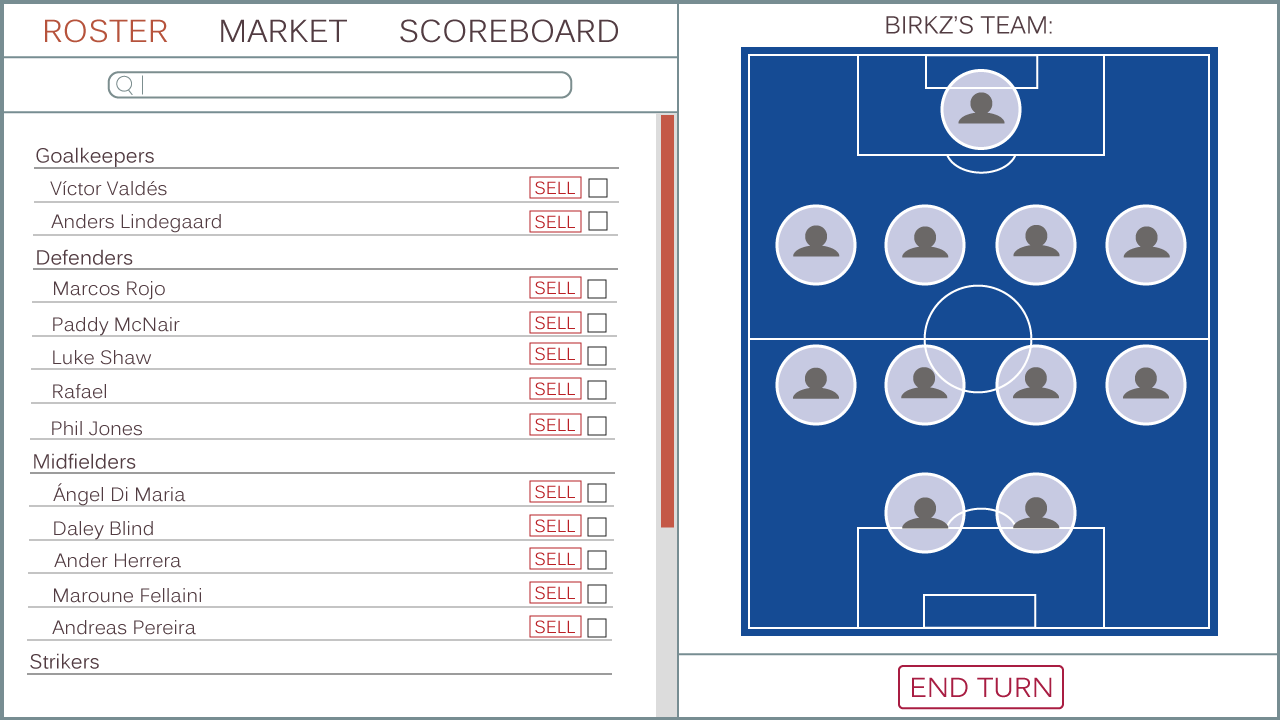
\includegraphics[width=0.99\textwidth]{ffUI.png}
\end{figure}


\end{document}